%*******************************************************************************
%****************************** Appendix E *************************************
%*******************************************************************************
\chapter{Additional results for HHI experiment} \label{appendix:e}


%% **************************** Define Graphics Path **************************
%\graphicspath{{chapter7/figs/raster/}{chapter7/figs/PDF/}{chapter7/figs/}}
\graphicspath{{figs/chapter6/PDF/}}


\LaTeX .cls  files can be accessed system-wide when they are placed in the
<texmf>/ tex/ latex directory, where <texmf> is the root directory of the user’s
\TeX installation.
On systems that have a local texmf tree (<texmflocal>), which
may be named ``texmf-local'' or ``localtexmf'', it may be advisable to install
packages in <texmflocal>, rather than <texmf> as the contents of the former,
unlike that of the latter, are preserved after the \LaTeX system is reinstalled
and/or upgraded.


\section{Time Series} \label{appendix:e:ts}


\section{Embedding parameters} \label{appendix:e:ep}



%%---------------------------------(FIGURE)-------------------------------------
%\begin{figure}[!h]
\begin{figure}
\centering
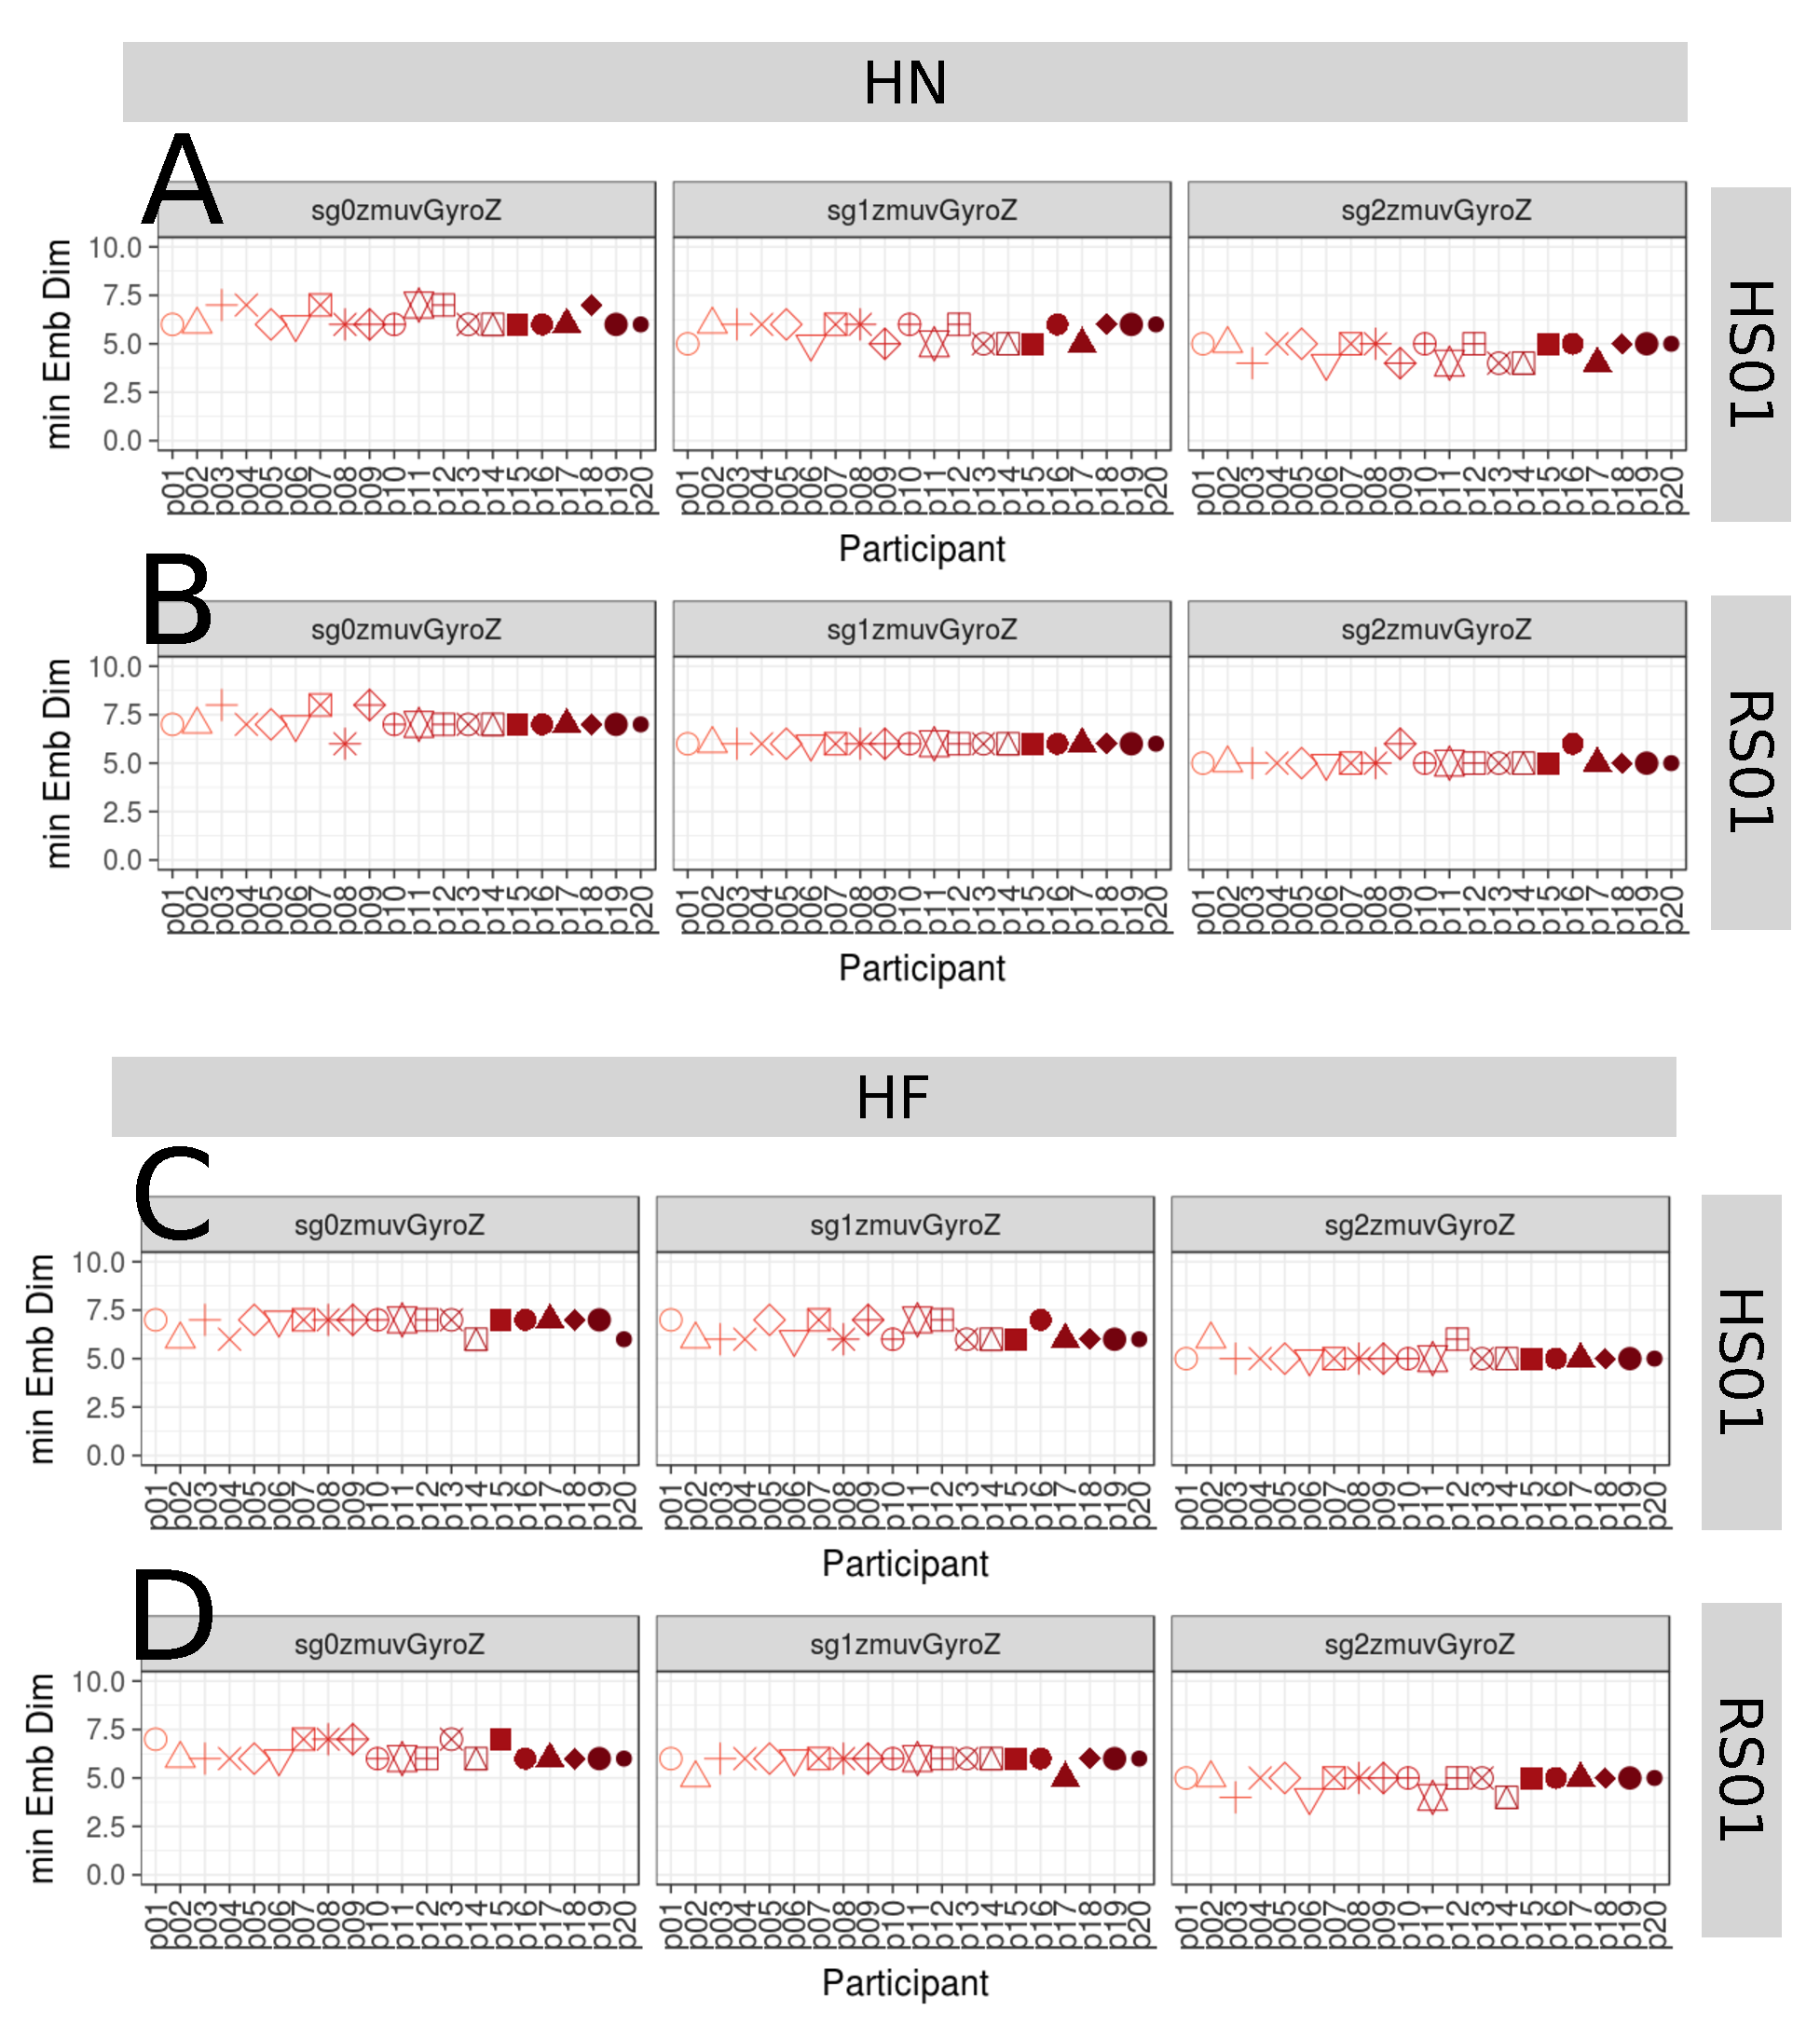
\includegraphics[width=1.0\textwidth]{cao_aHw10}
	\caption{
	{\bf Minimum embedding dimensions for horizontal arm movements.} 
		(A, B) Horizontal Normal (HN), (C, D) Horizontal Faster (HF) 
		movements,
		(A, C) sensor attached to participants (HS01), and
		(B, D) sensor attached to robot (RS01).
		Minimum embedding dimensions are for twenty participants 
		(p01 to p20) with three smoothed signals 
		(sg0zmuvGyroZ, sg1zmuvGyroZ and sg2zmuvGyroZ)
		and window lenght of 10-sec (500 samples).
		R code to reproduce the figure is available 
		from \cite{hwum2018}.
        }
    \label{fig:caoH}
\end{figure}
%%---------------------------------(FIGURE)------------------------------------

%%---------------------------------(FIGURE)-------------------------------------
%\begin{figure}[!h]
\begin{figure}
\centering
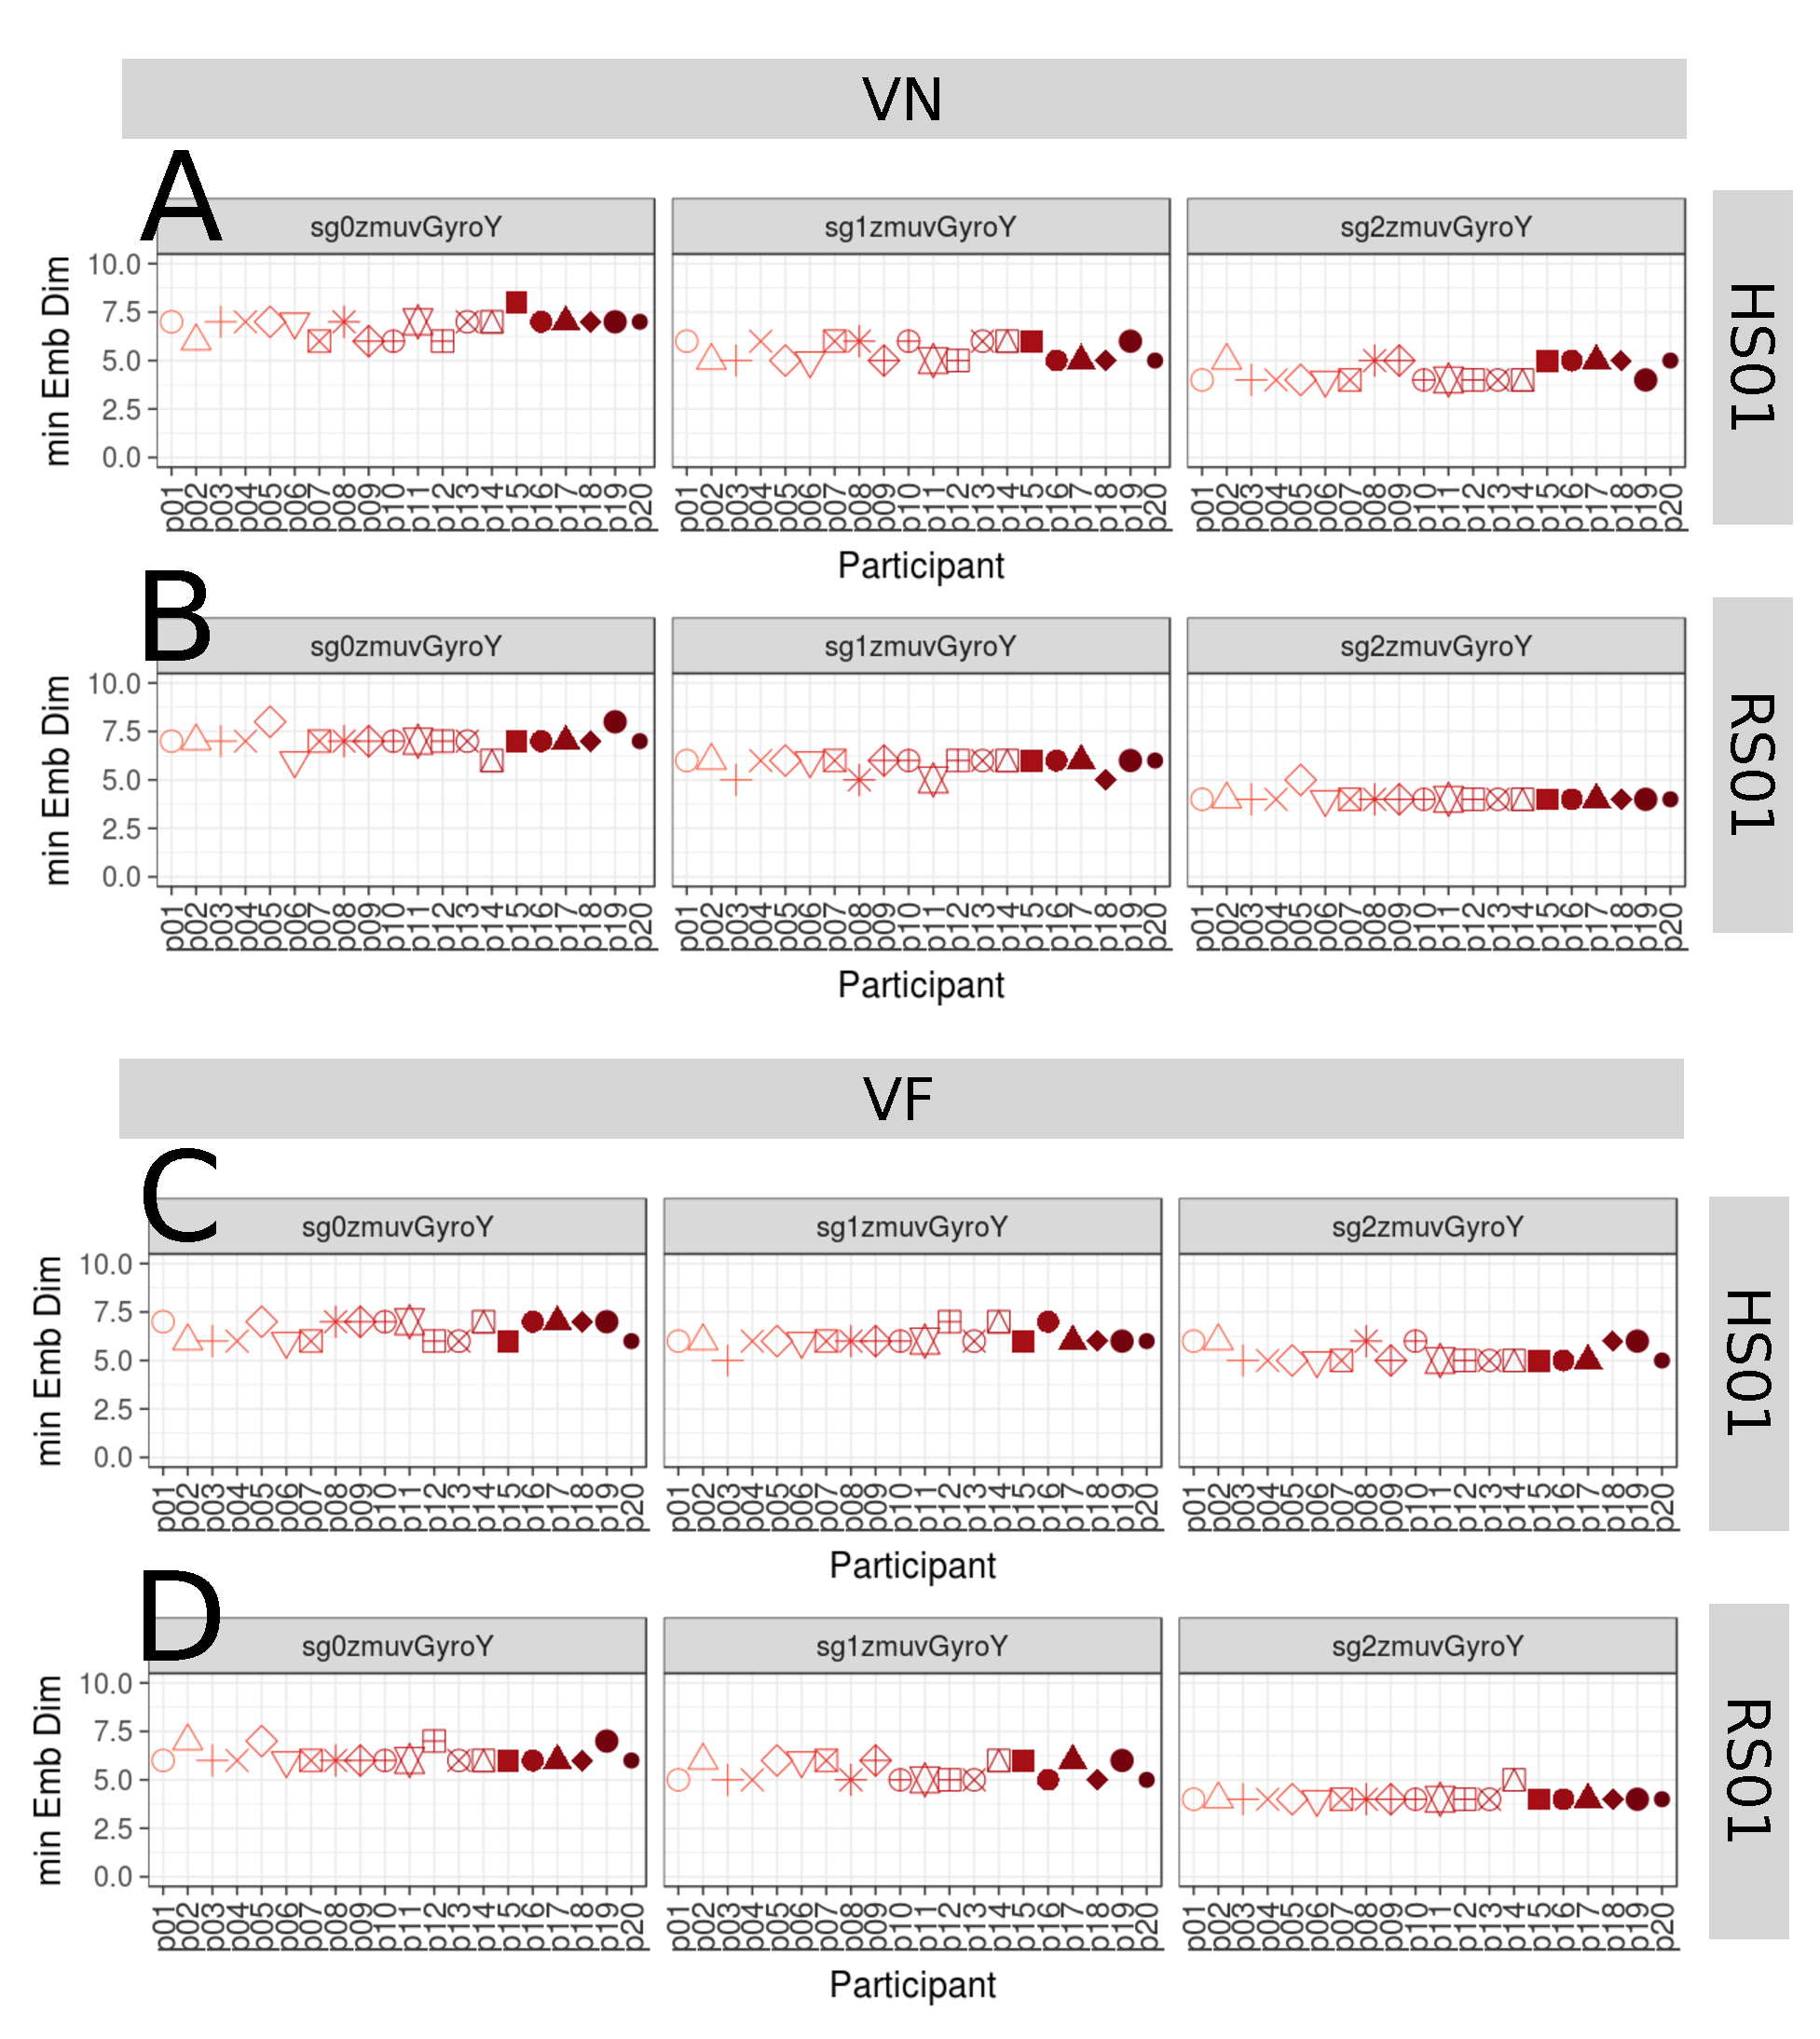
\includegraphics[width=1.0\textwidth]{cao_aVw10}
	\caption{
	{\bf Minimum embedding dimensions for vertical arm movements.} 
		(A, B) Vertical Normal (VN), (C, D) Vertical Faster (VF) 
		movements,
		(A, C) sensor attached to participants (HS01), and		
		(B, D) sensor attached to robot (RS01).
		Minimum embedding dimensions are for twenty participants 
		(p01 to p20) with three smoothed signals (sg0zmuvGyroY, 
		sg1zmuvGyroY and sg2zmuvGyroY) 
		and window length of 10-sec (500 samples).
		R code to reproduce the figure is available 
		from \cite{hwum2018}.
        }
    \label{fig:caoV}
\end{figure}
%%---------------------------------(FIGURE)------------------------------------



%%---------------------------------(FIGURE)-------------------------------------
%\begin{figure}[!h]
\begin{figure}
\centering
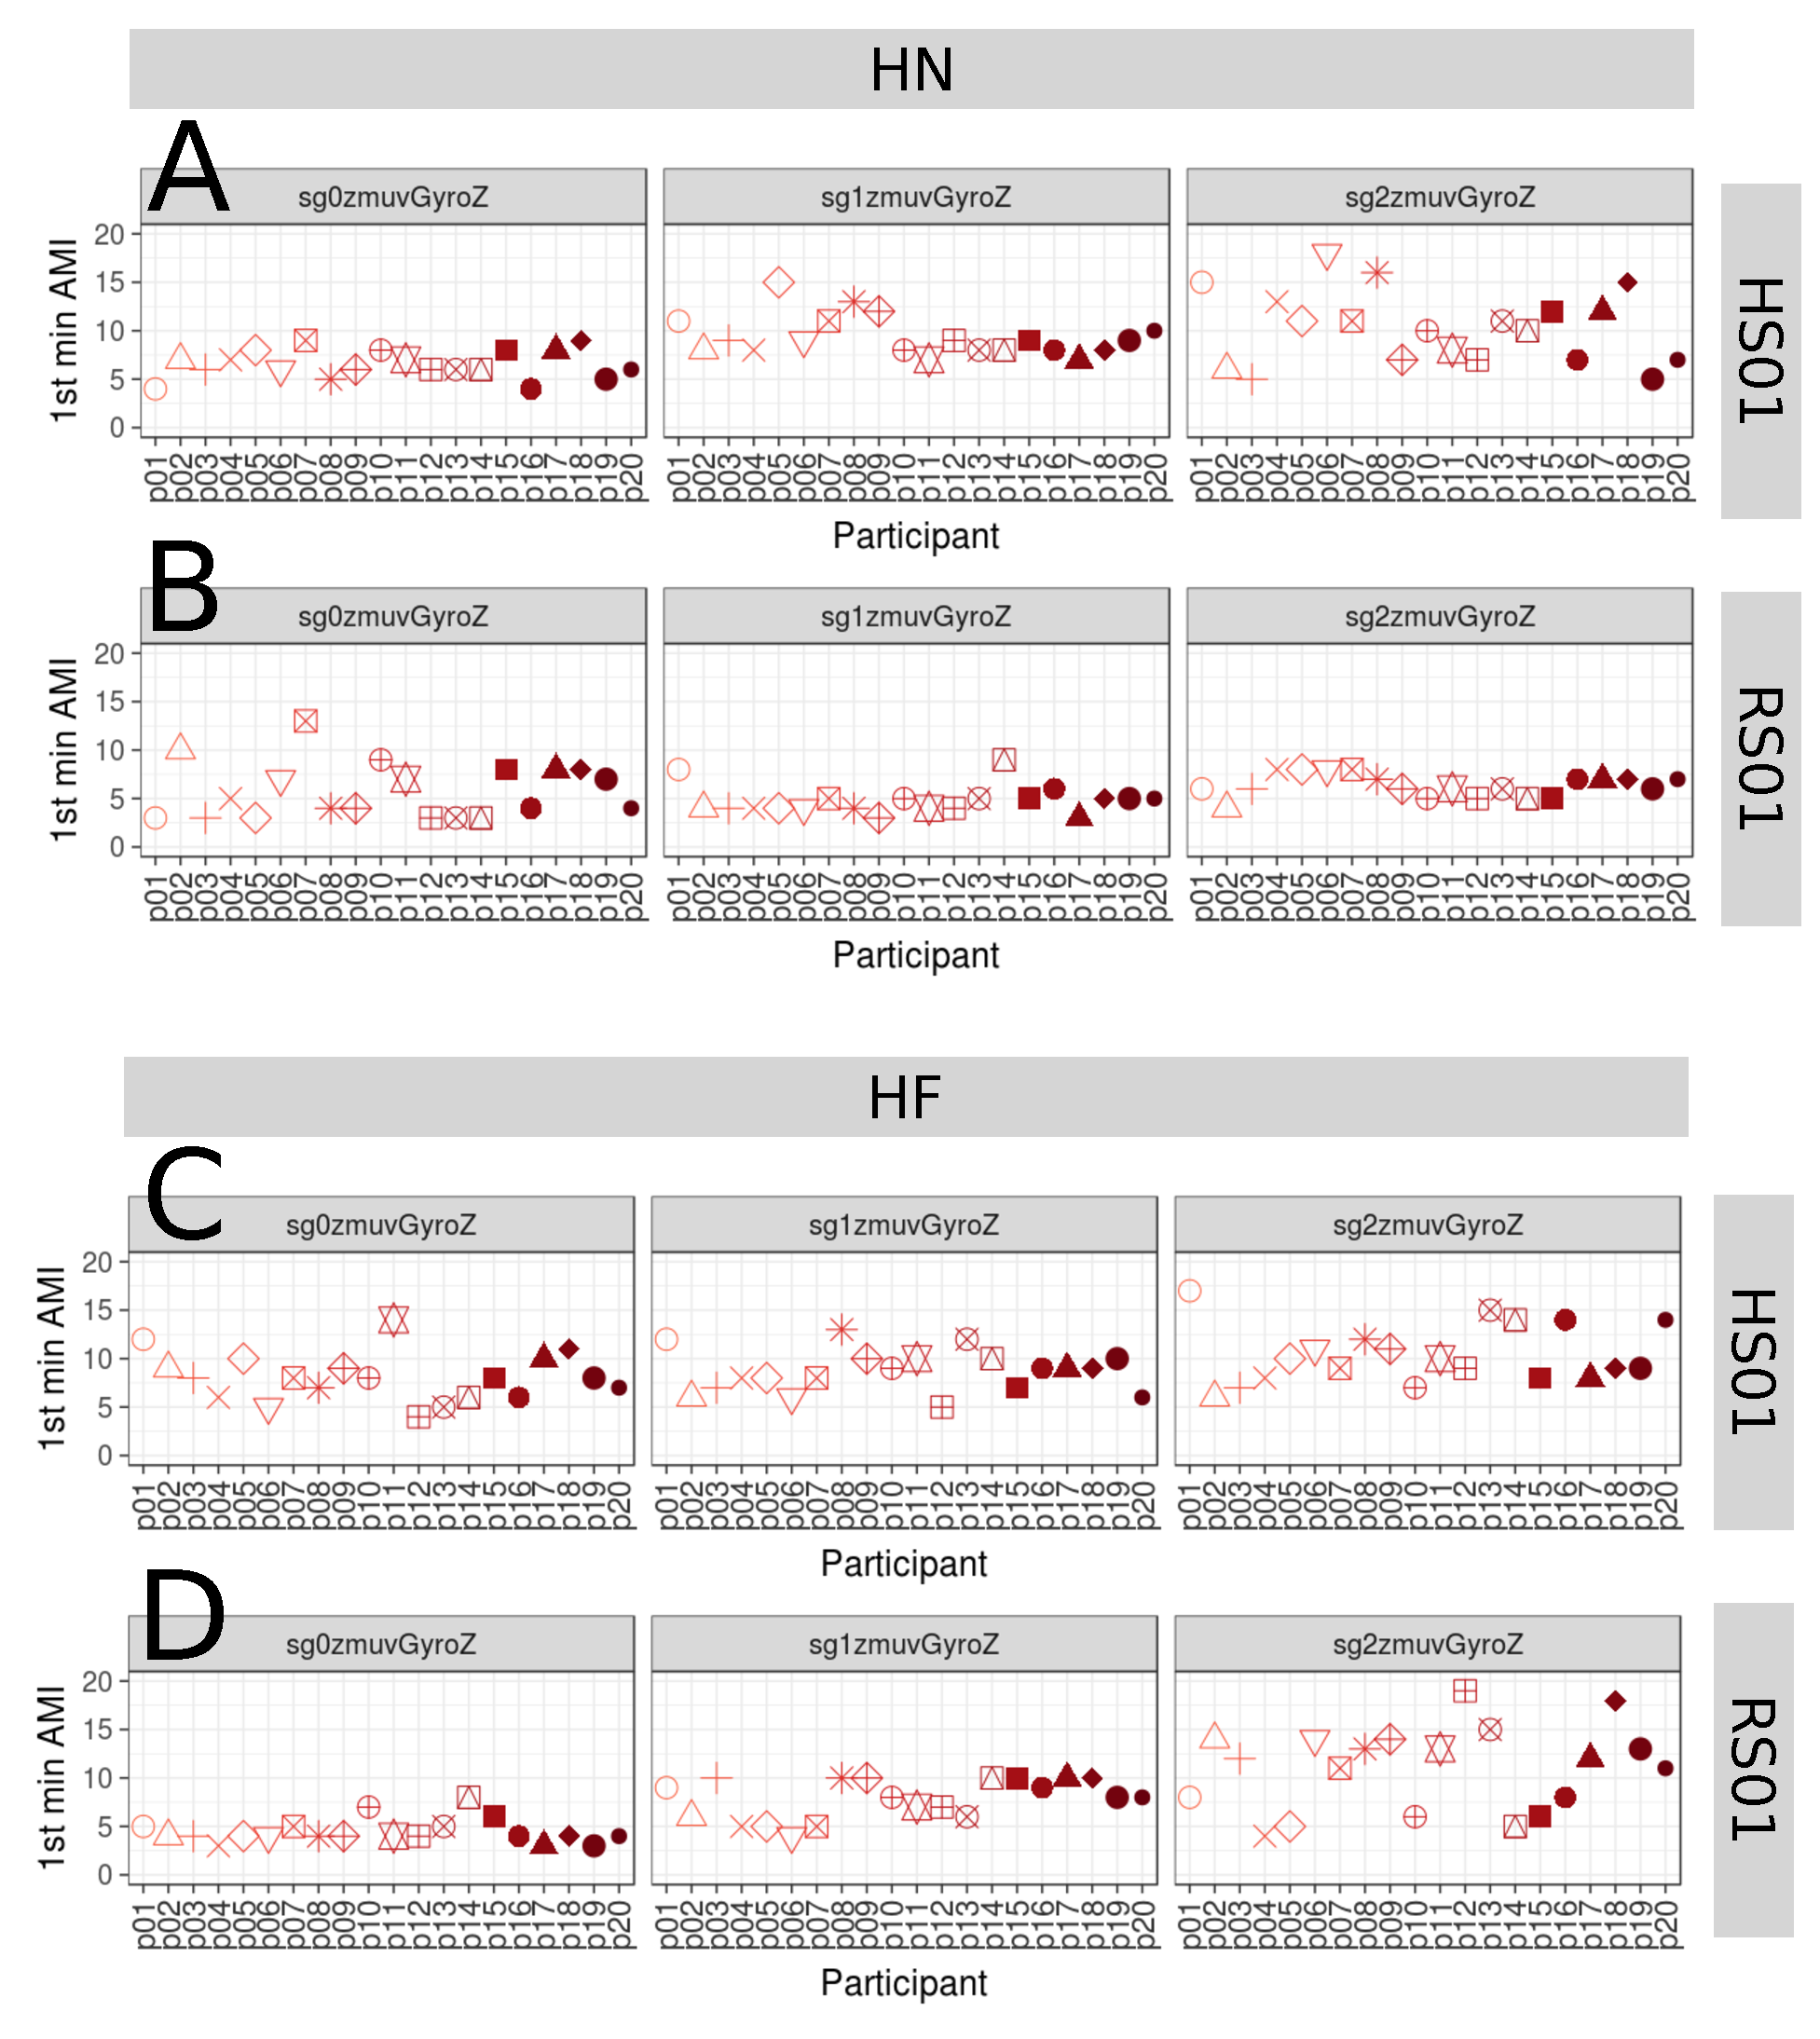
\includegraphics[width=1.0\textwidth]{ami_aHw10}
	\caption{
	{\bf First minimum AMI values for horizontal arm movements.}
		(A, B) Horizontal Normal (HN), (C, D) Horizontal Faster (HF) 
		movements,
		(A, C) sensor attached to participants (HS01), and
		(B, D) sensor attached to robot (RS01).
		First minimum AMI values are for twenty participants 
		(p01 to p20) with three smoothed signals (sg0zmuvGyroZ, 
		sg1zmuvGyroZ and sg2zmuvGyroZ) and  window lenght of 
		10-sec (500 samples).
		R code to reproduce the figure is available 
		from \cite{hwum2018}.
        }
    \label{fig:amiH}
\end{figure}
%%---------------------------------(FIGURE)------------------------------------

%%---------------------------------(FIGURE)-------------------------------------
%\begin{figure}[!h]
\begin{figure}
\centering
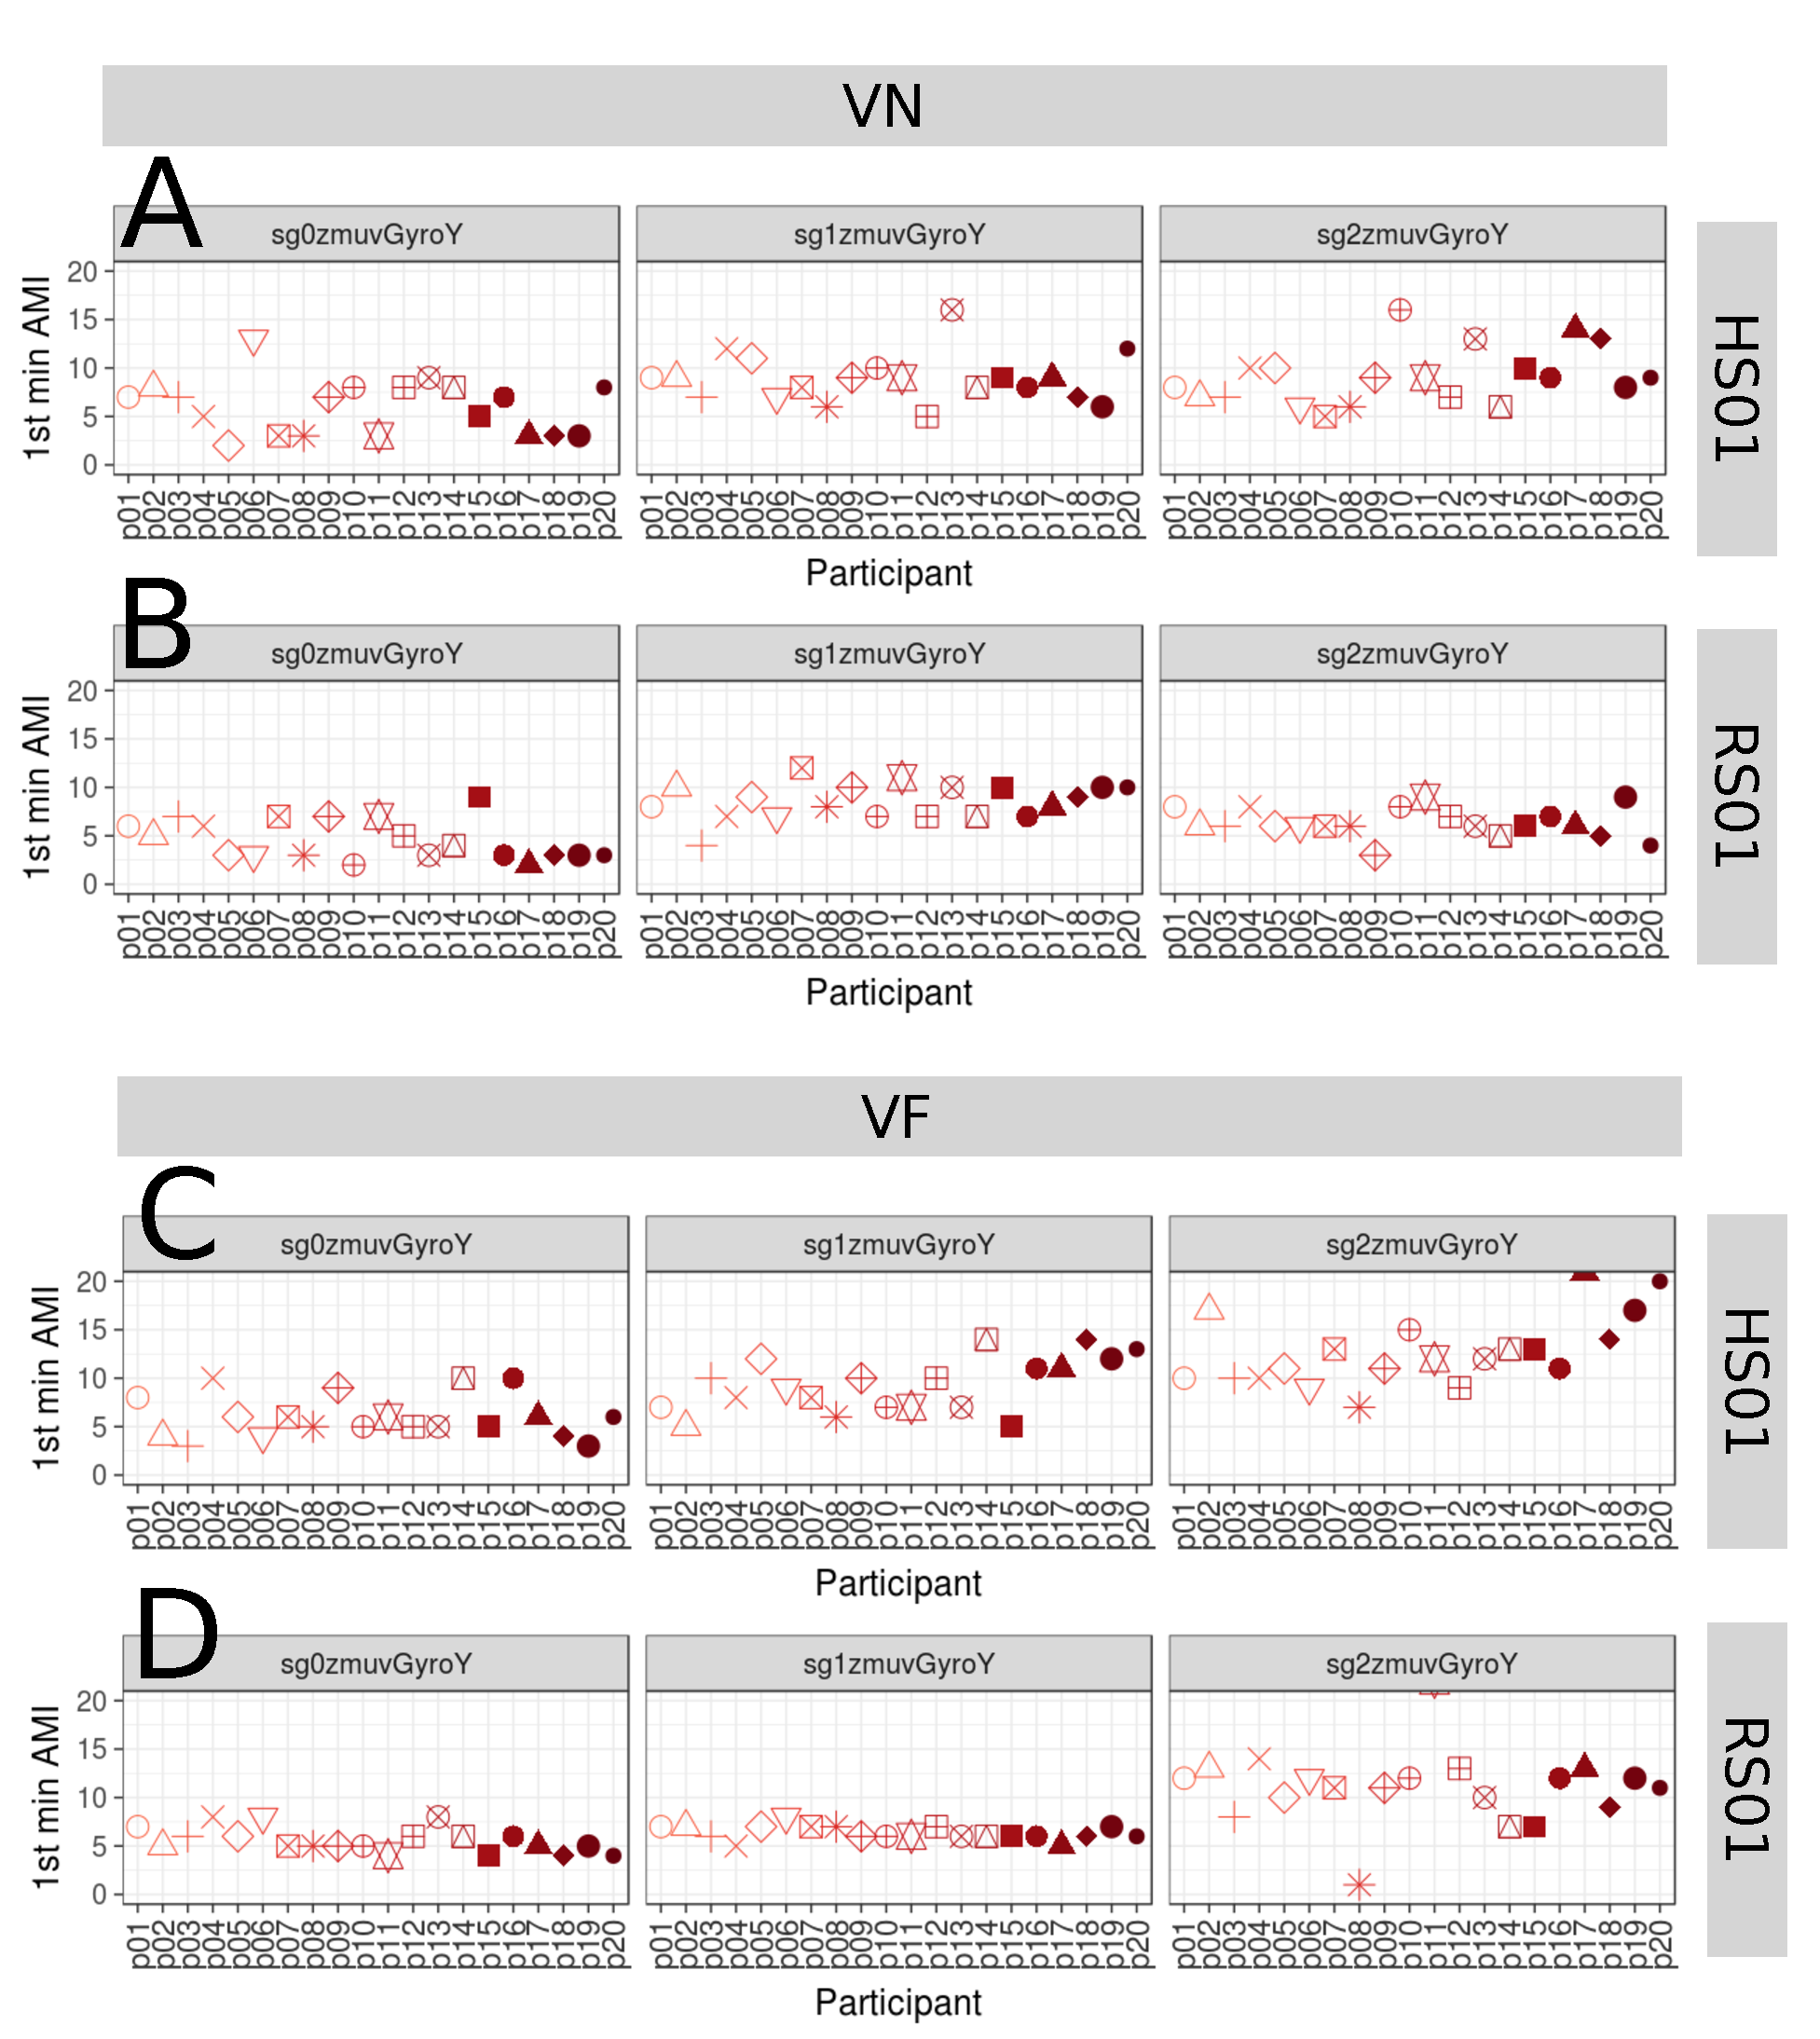
\includegraphics[width=1.0\textwidth]{ami_aVw10}
	\caption{
	{\bf First minimum AMI values for vertical arm movements.}
		(A, B) Vertical Normal (VN), (C, D) Vertical Faster (VF) 
		movements,
		(A, C) sensor attached to participants (HS01), and
		(B, D) sensor attached to robot (RS01).
		First minimum AMI values are for twenty participants 
		(p01 to p20) with three smoothed signals (sg0zmuvGyroZ, 
		sg1zmuvGyroZ and sg2zmuvGyroZ) and  window lenght of 
		10-sec (500 samples).
		R code to reproduce the figure is available 
		from \cite{hwum2018}.
        }
    \label{fig:amiV}
\end{figure}
%%---------------------------------(FIGURE)------------------------------------




\section{RSSs} \label{appendix:e:rsss}
\section{RPs} \label{appendix:e:rps}


\section{RQAs} \label{appendix:e:rpas}

\subsection{REC values}
It can be seen in Figs~\ref{fig:rec_aH} and \ref{fig:rec_aV} 
that REC values, representing the \% of black dots in the RPs, 
are more spread for HN than HF movements with time 
series coming from HS01 sensor. 
In contrast, REC values appear to be constant and present little variation 
for both HN and HF movements with time series from the sensor attached 
to the humanoid robot RS01.
With regard to the increase of smoothness of time series 
(sg0zmuvGyroZ, sg1zmuvGyroZ and sg2zmuvGyroZ), REC values present little 
variation as the smoothness is increasing for time series from HS01 and 
REC values more similar as the smoothness is increasing for data from RS01.


%%---------------------------------(FIGURE)-------------------------------------
\begin{figure}[!h]
\centering
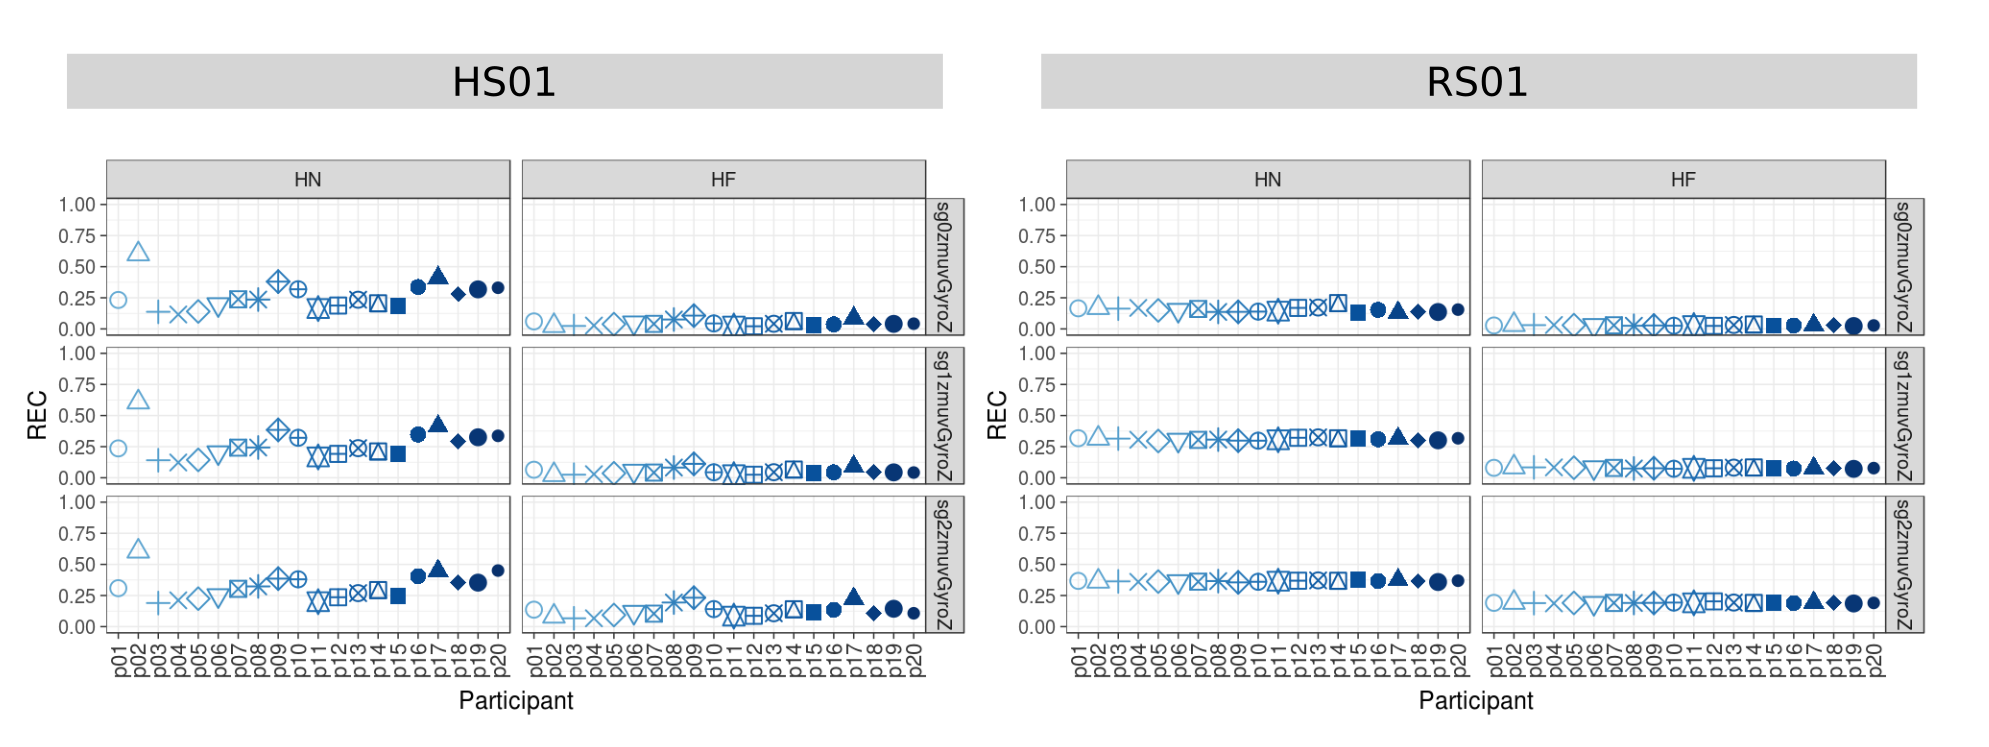
\includegraphics[width=1.0\textwidth]{rec_aH}
    \caption{
	{\bf REC values for horizontal arm movements.}	
	REC values (representing \% of black dots in the RPs) for 
	20 participants performing HN and HF movements
	with sensors HS01, RS01 and three smoothed-normalised axis 
	of GyroZ (sg0zmuvGyroZ, sg1zmuvGyroZ and sg2zmuvGyroZ).
	REC values were computed with 
	embedding parameters $m=6$, $\tau=8$ and $\epsilon=1$
	R code to reproduce the figure is available from \cite{hwum2018}.
        }
    \label{fig:rec_aH}
\end{figure}
%%---------------------------------(FIGURE)------------------------------------
%%---------------------------------(FIGURE)-------------------------------------
\begin{figure}[!h]
\centering
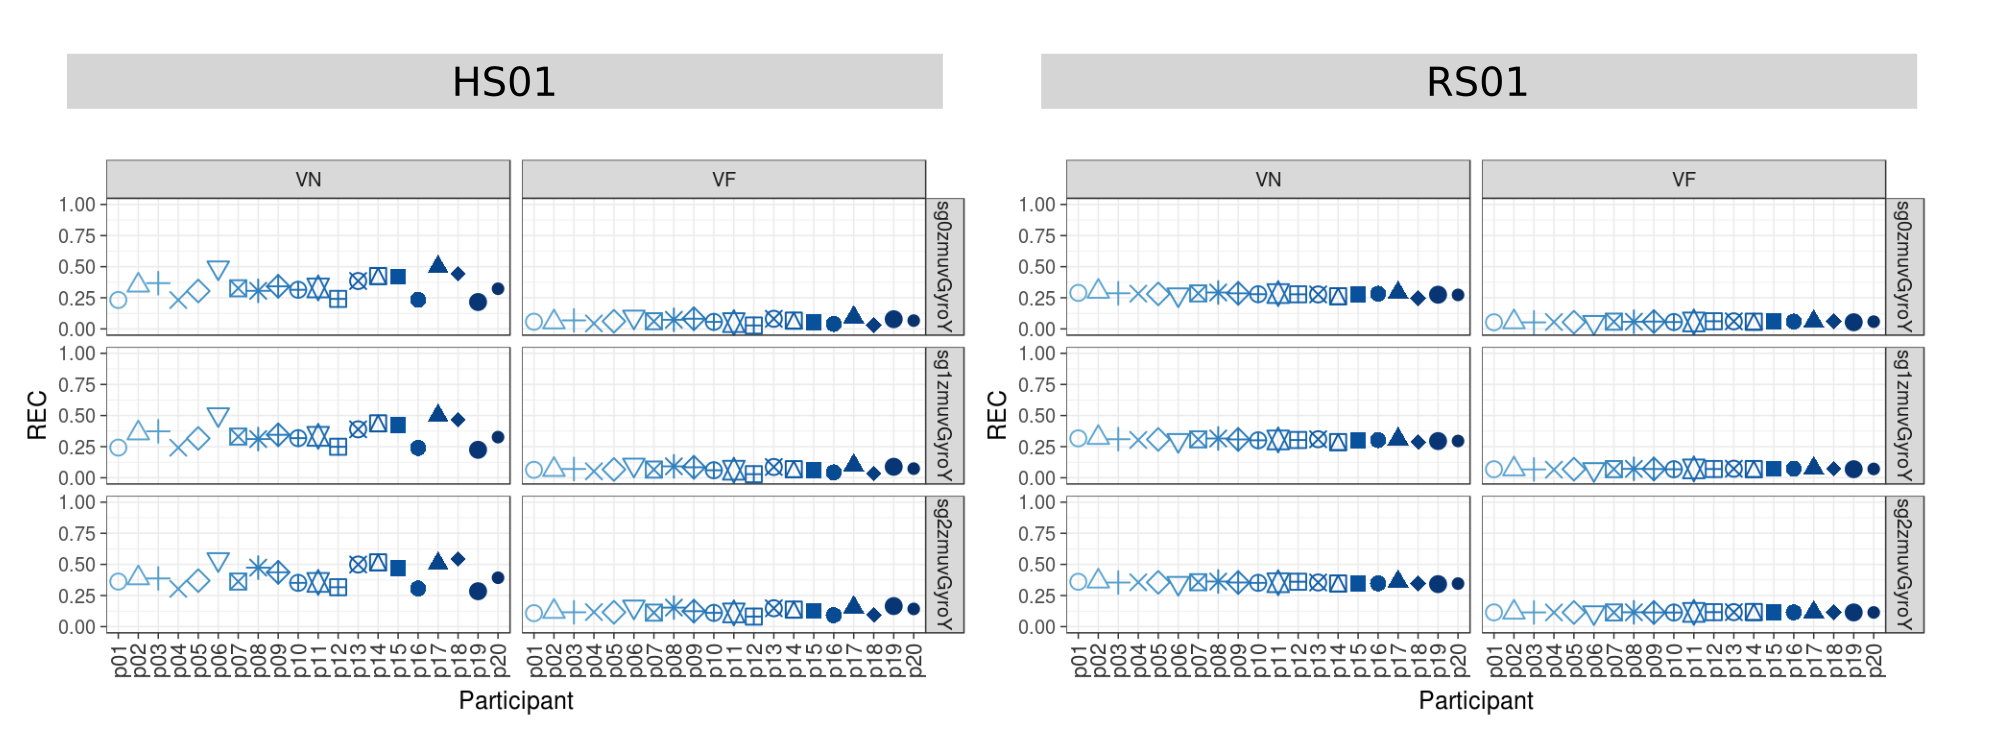
\includegraphics[width=1.0\textwidth]{rec_aV}
    \caption{
	{\bf REC values for vertical arm movements.}	
	REC values (representing \% of black dots in the RPs) for 
	20 participants performing VN and VF movements
	with sensors HS01, RS01 and three smoothed-normalised axis 
	of GyroY (sg0zmuvGyroY, sg1zmuvGyroY and sg2zmuvGyroY).
	REC values were computed with 
	embedding parameters $m=6$, $\tau=8$ and $\epsilon=1$.
	R code to reproduce the figure is available from \cite{hwum2018}.
        }
    \label{fig:rec_aV}
\end{figure}
%%---------------------------------(FIGURE)------------------------------------


\subsection{DET values}
DET values, representing predictability and organisation of the RPs, 
change very little even for type of movement and type of sensor
(Figs~\ref{fig:det_aH} and \ref{fig:det_aV}).
With regard to the smoothness of time series, DET values appear 
to be more similar as the smoothness of the time series is increasing.
%%---------------------------------(FIGURE)-------------------------------------
\begin{figure}[!h]
\centering
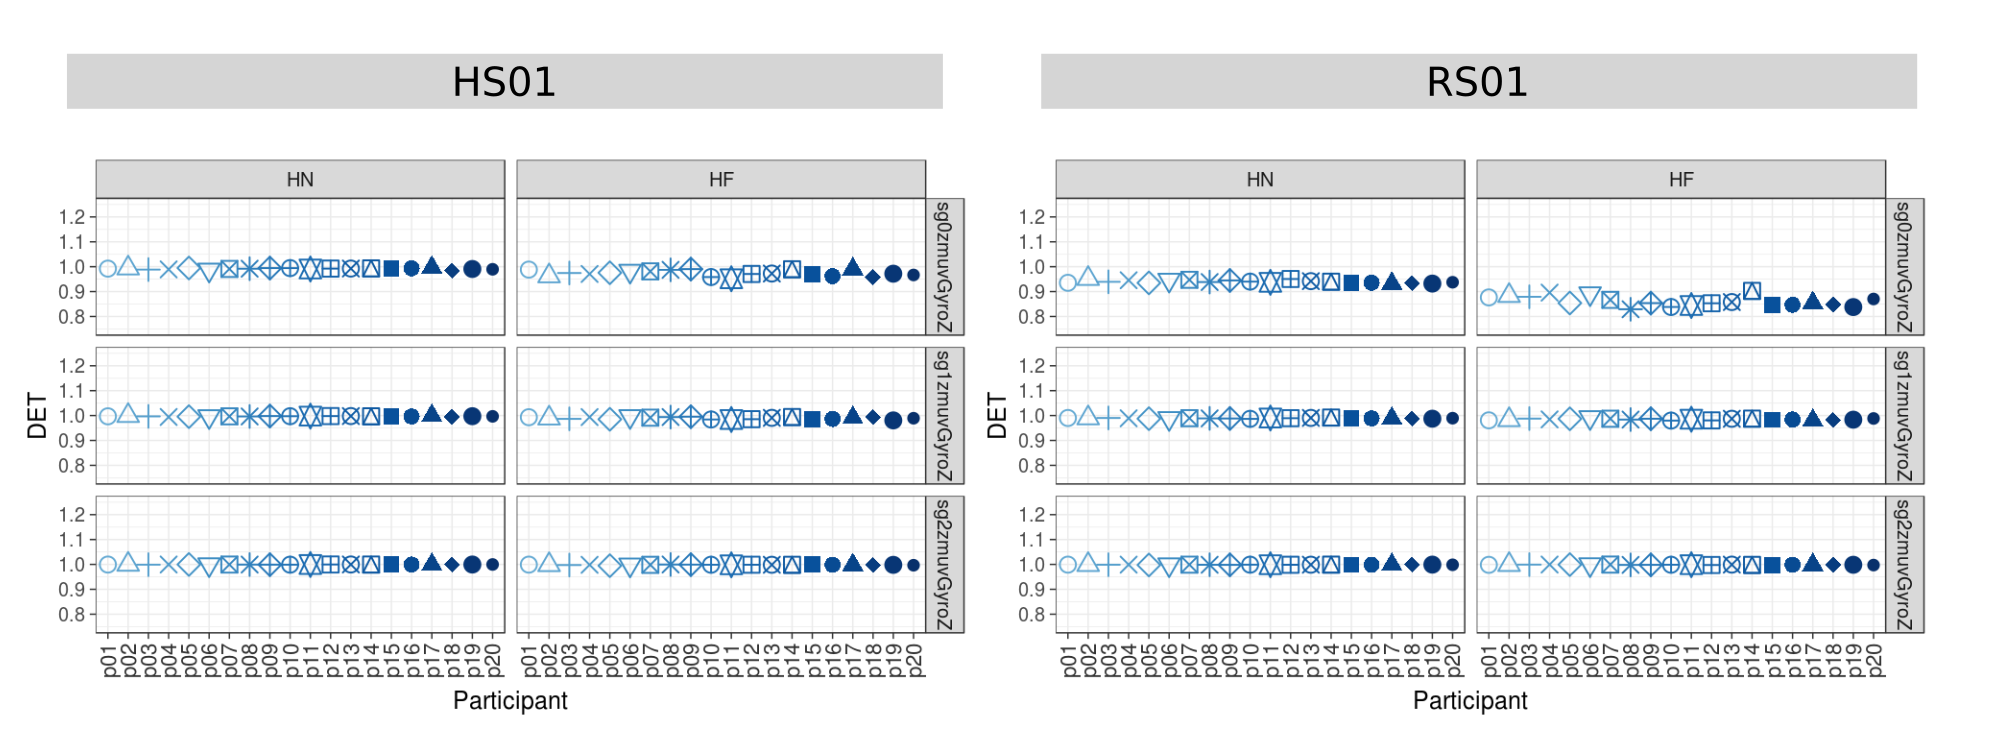
\includegraphics[width=1.0\textwidth]{det_aH}
    \caption{
	{\bf DET values for horizontal arm movements.}	
    	DET values (representing predictability and organisation of the RPs)
	for 20 participants performing HN and HF movements
	with sensors HS01, RS01 and three smoothed-normalised axis 
	of GyroZ (sg0zmuvGyroZ, sg1zmuvGyroZ and sg2zmuvGyroZ).
	DET values were computed with 
	embedding parameters $m=6$, $\tau=8$ and $\epsilon=1$.
	R code to reproduce the figure is available from \cite{hwum2018}.
        }
    \label{fig:det_aH}
\end{figure}
%%---------------------------------(FIGURE)------------------------------------
%%---------------------------------(FIGURE)-------------------------------------
\begin{figure}[!h]
\centering
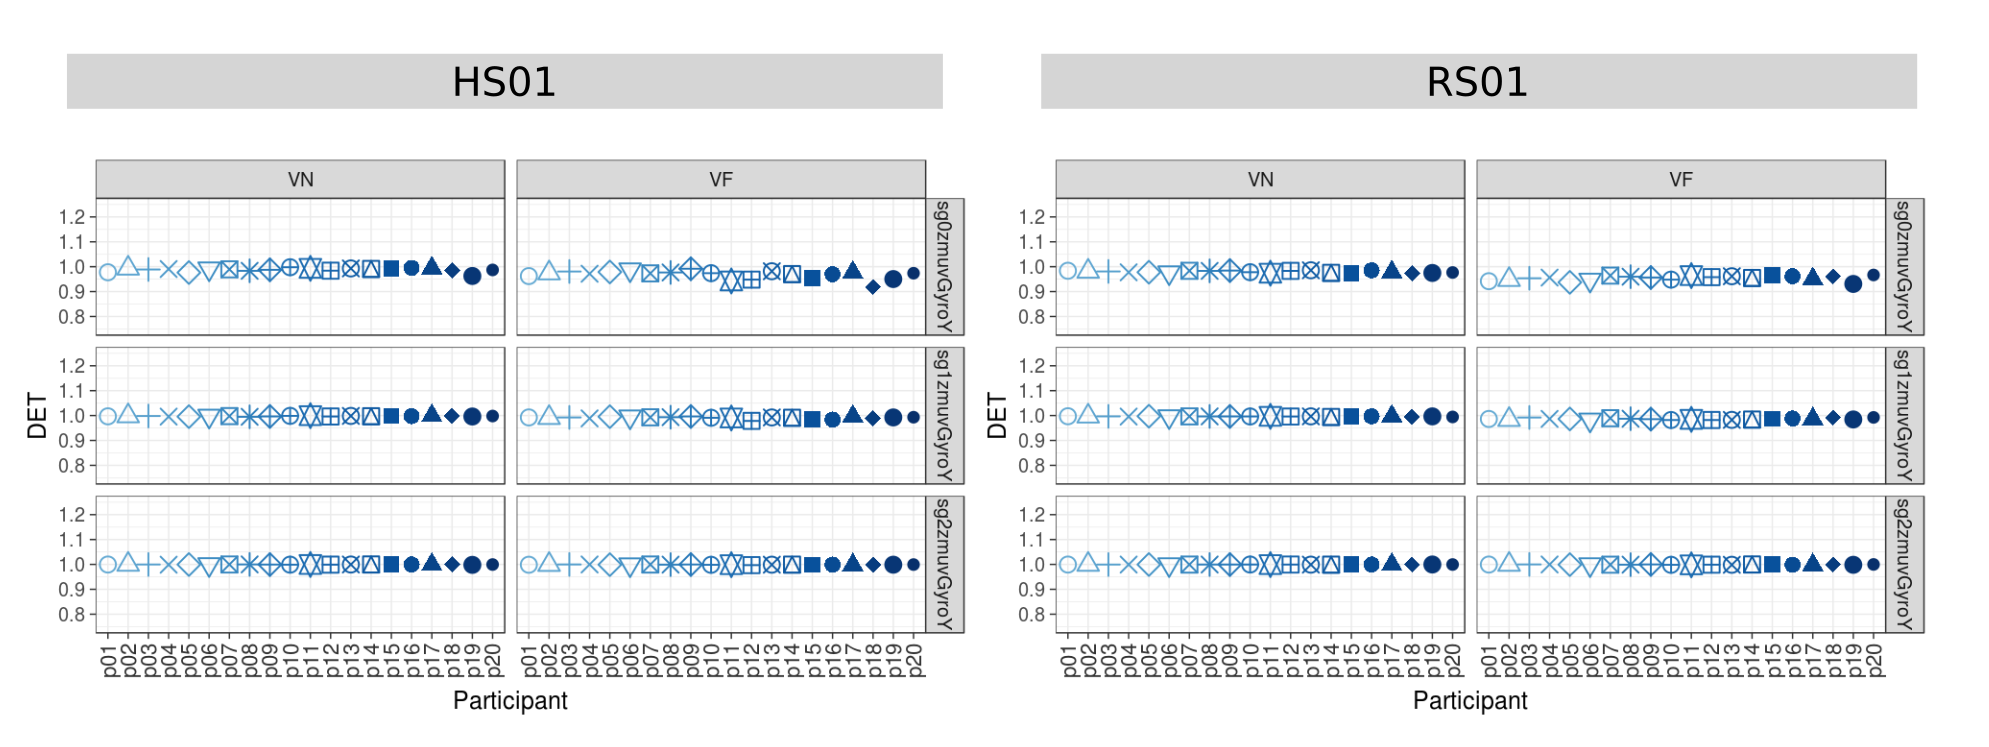
\includegraphics[width=1.0\textwidth]{det_aV}
    \caption{
	{\bf DET values for vertical arm movements.}	
    	DET values (representing predictability and organisation of the RPs) 
	for 20 participants performing VN and VF movements
	with sensors HS01, RS01 and three smoothed-normalised axis 
	of GyroY (sg0zmuvGyroY, sg1zmuvGyroY and sg2zmuvGyroY).
	DET values were computed with 
	embedding parameters $m=6$, $\tau=8$ and $\epsilon=1$.
	R code to reproduce the figure is available from \cite{hwum2018}.
        }
    \label{fig:det_aV}
\end{figure}
%%---------------------------------(FIGURE)------------------------------------



\subsection{RATIO values}
RATIO values, representing dynamic transitions, for both horizontal and
vertical movements (Figs~\ref{fig:ratio_aH} and \ref{fig:ratio_aV})
vary less for HN movements than HF movements for HS01 sensor 
which is a similar behaviour of RATIO values for RS01 sensor.
It can also noticed a decrease of variation in RATIO values as the 
smoothness of the time series is increasing.
%%---------------------------------(FIGURE)-------------------------------------
\begin{figure}[!h]
\centering
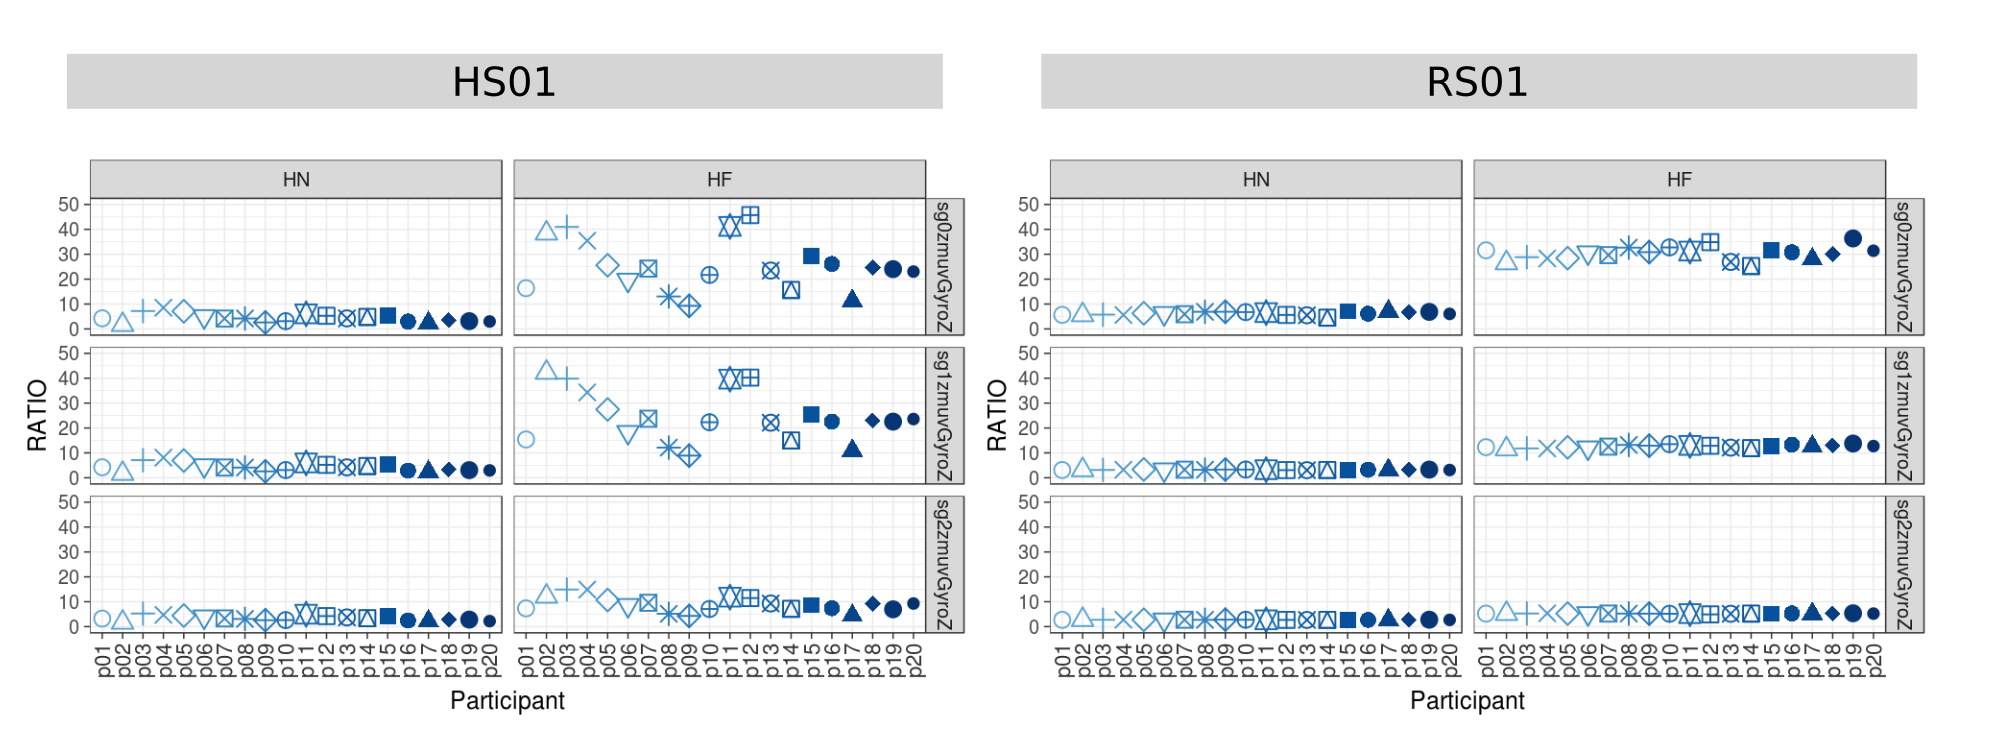
\includegraphics[width=1.0\textwidth]{ratio_aH}
    \caption{
	{\bf RATIO values for horizontal arm movements.}
	RATIO (representing dynamic transitions) for 
	20 participants performing HN and HF movements
	with sensors HS01, RS01 and three smoothed-normalised axis 
	of GyroZ (sg0zmuvGyroZ, sg1zmuvGyroZ and sg2zmuvGyroZ).
	RATIO values were computed with 
	embedding parameters $m=6$, $\tau=8$ and $\epsilon=1$.
	R code to reproduce the figure is available from \cite{hwum2018}.
        }
    \label{fig:ratio_aH}
\end{figure}
%%---------------------------------(FIGURE)------------------------------------
%%---------------------------------(FIGURE)-------------------------------------
\begin{figure}[!h]
\centering
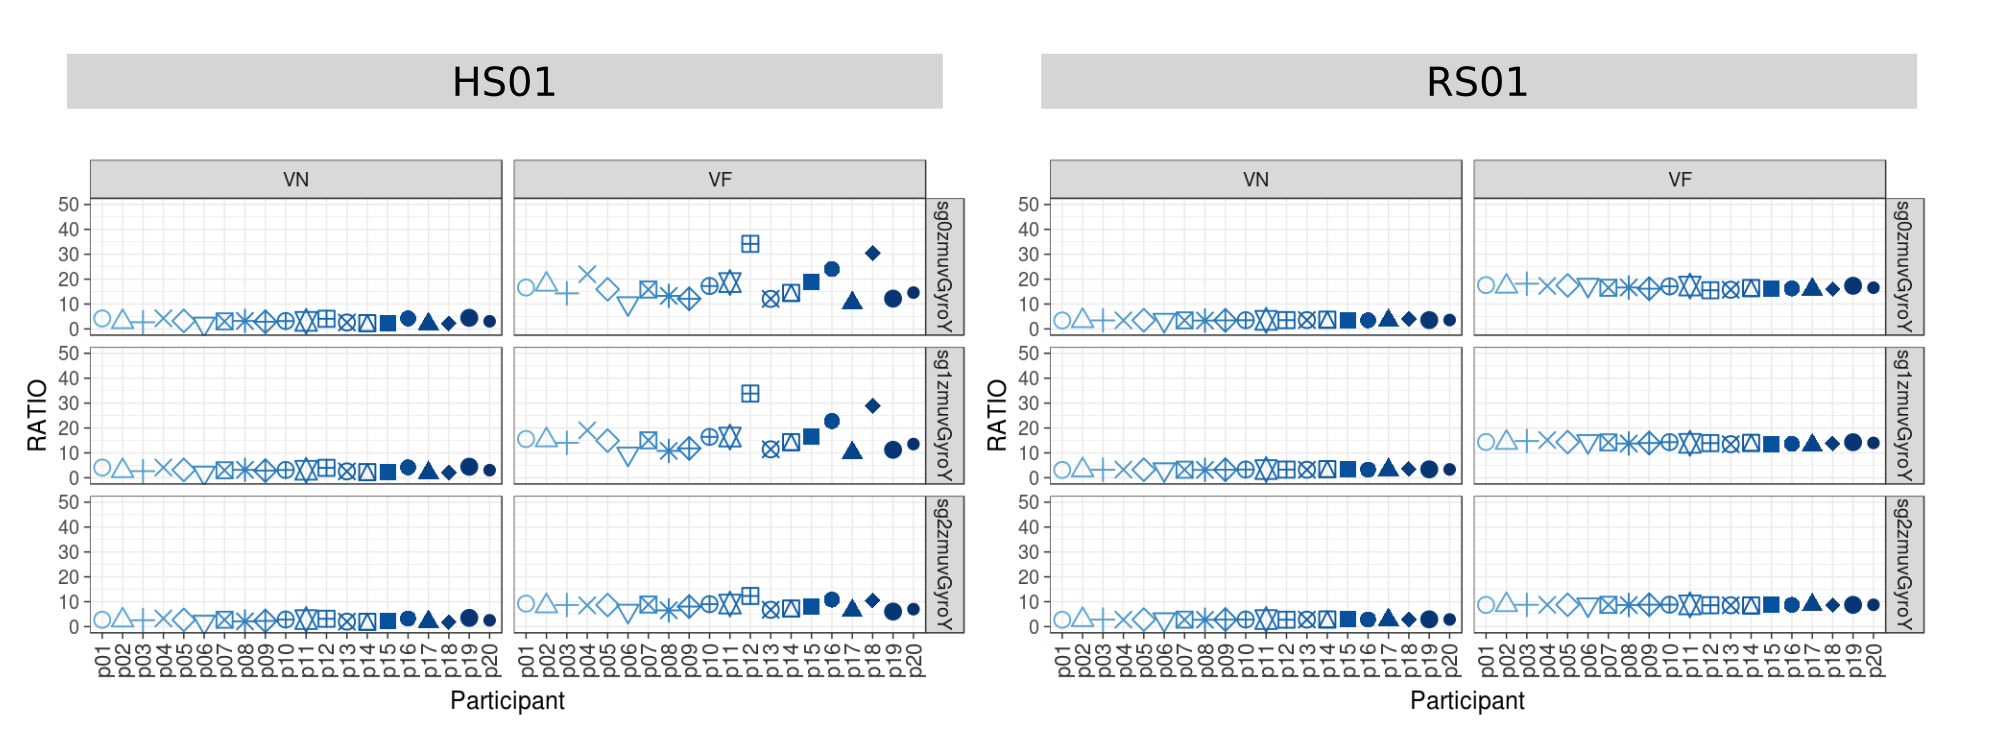
\includegraphics[width=1.0\textwidth]{ratio_aV}
    \caption{
	{\bf RATIO values for vertical arm movements.}
	RATIO (representing dynamic transitions) for 
	20 participants performing VN and VF movements
	with sensors HS01, RS01 and three smoothed-normalised axis 
	of GyroY (sg0zmuvGyroY, sg1zmuvGyroY and sg2zmuvGyroY).
	RATIO values were computed with
	embedding parameters $m=6$, $\tau=8$ and $\epsilon=1$.
	R code to reproduce the figure is available from \cite{hwum2018}.
        }
    \label{fig:ratio_aV}
\end{figure}
%%---------------------------------(FIGURE)------------------------------------



\subsection{ENTR values}
ENTR values, representing the complexity of the deterministic structure 
of the time series, for both horizontal and vertical movements 
(Figs~\ref{fig:entr_aH} and \ref{fig:entr_aV}) show more variation 
for HS01 sensor than ENTR values for RS01 sensor which appear 
to be more constant. 
Generally, it can also be said that the smoothness of time series affects 
little to the variation of ENTR values.
%%---------------------------------(FIGURE)-------------------------------------
\begin{figure}[!h]
\centering
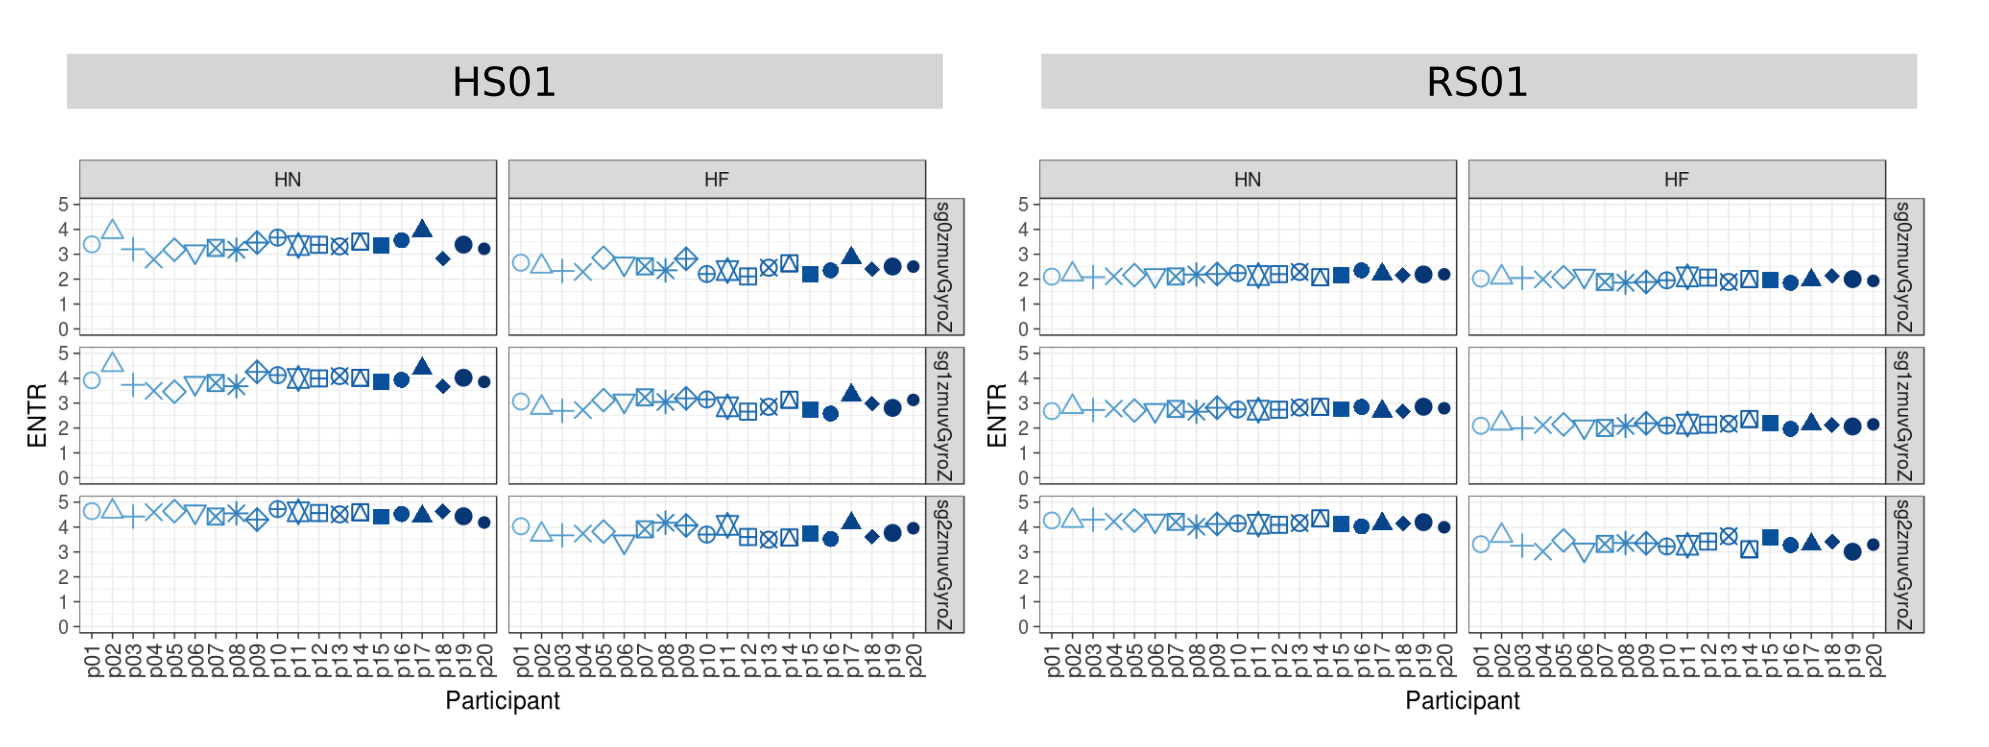
\includegraphics[width=1.0\textwidth]{entr_aH}
    \caption{
	{\bf ENTR values for horizontal arm movements.}
    	ENTR values (representing the complexity of the deterministic 
	structure in time series) for 
	20 participants performing HN and HF movements
	with sensors HS01, RS01 and three smoothed-normalised axis 
	of GyroZ (sg0zmuvGyroZ, sg1zmuvGyroZ and sg2zmuvGyroZ).
	ENTR values were computed with 
	embedding parameters $m=6$, $\tau=8$ and $\epsilon=1$.
	R code to reproduce the figure is available from \cite{hwum2018}.
        }
    \label{fig:entr_aH}
\end{figure}
%%---------------------------------(FIGURE)------------------------------------
%%---------------------------------(FIGURE)-------------------------------------
\begin{figure}[!h]
\centering
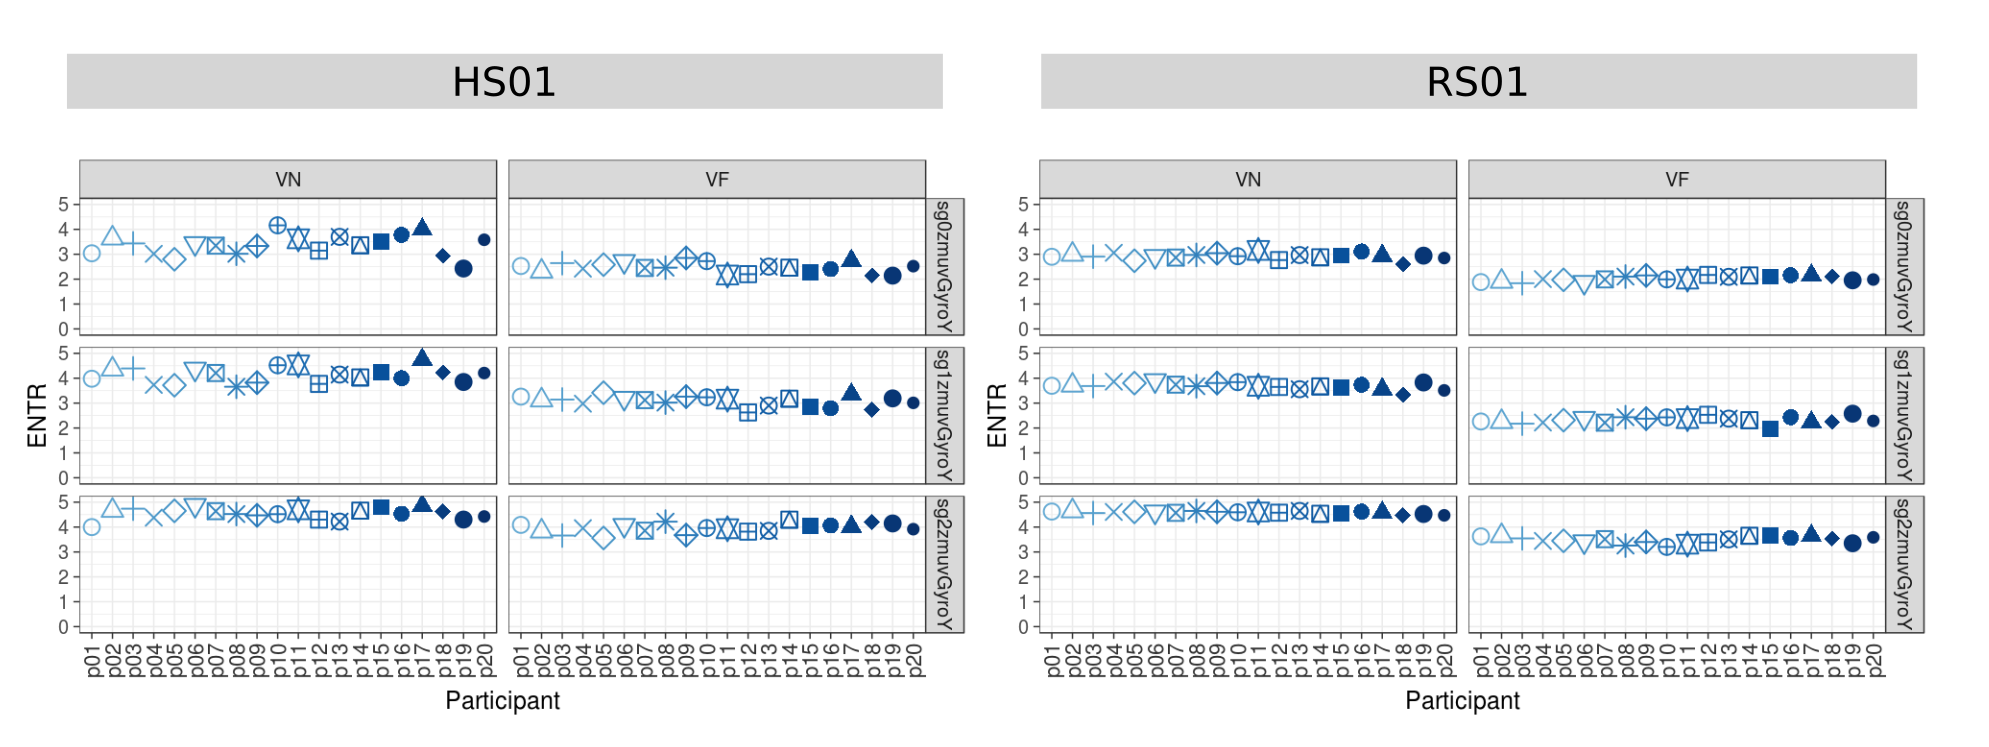
\includegraphics[width=1.0\textwidth]{entr_aV}
    \caption{
	{\bf ENTR values for vertical arm movements.}
    	ENTR values (representing the complexity of the deterministic 
	structure in time series) for 
	20 participants performing VN and VF movements
	with sensors HS01, RS01 and three smoothed-normalised axis 
	of GyroY (sg0zmuvGyroY, sg1zmuvGyroY and sg2zmuvGyroY).
	ENTR values were computed with 
	embedding parameters $m=6$, $\tau=8$ and $\epsilon=1$.
	R code to reproduce the figure is available from \cite{hwum2018}.
        }
    \label{fig:entr_aV}
\end{figure}
%%---------------------------------(FIGURE)------------------------------------





